%   % !TEX root = ../../VIII,3_Rahmen-TeX_8-1.tex
%
%
%   Band VIII, 3 N.~??A34.1
%   Signatur/Tex-Datei: LH_35_14_02_162r
%   RK-Nr. 58256 [Teil 2 ??]
%   Überschrift: [Chordae extensae restitutionis velocitas]
%   Modul: Mechanik / AEF (Elastizität)
%   Datierung: [Anfang August bis zweite Hälfte November 1689]
%   WZ: LEdWZ 803044 = RK-WZ 125 // 40l
%   SZ: (keins)
%   Bilddateien (PDF): LH_35_14_02_162r_d1; LH_35_14_02_162r_d2 (insgesamt: zwei)
%
%
\selectlanguage{ngerman}%
\frenchspacing%
%
\begin{ledgroupsized}[r]{120mm}
\footnotesize
\pstart
\noindent\textbf{Überlieferung:}
\pend
\end{ledgroupsized}
\begin{ledgroupsized}[r]{114mm}
\footnotesize
\pstart \parindent -6mm
\makebox[6mm][l]{\textit{L}}%
Aufzeichnung:
LH~XXXV~14, 2 Bl.~161\textendash162.
Ein Bogen 8\textsuperscript{o};
Fragment eines Wasserzeichens auf Bl.~162:
italienisches Papier.
Eine Seite auf Bl.~162~r\textsuperscript{o}\! und fünf Zeilen auf Bl.~161~v\textsuperscript{o}.
Bl.~162~v\textsuperscript{o}, 161~r\textsuperscript{o} und 161~v\textsuperscript{o}\! überliefern N.~28\textsubscript{2}.
Bl.~162~r\textsuperscript{o} überliefert ferner, quer zur Schreib\-rich\-tung und überschrieben, folgendes mit dem Briefkonzept \textit{LSB} I,~5 N.~250\cite{01297} % (bes. S.~46.8\textendash10) 
zusammenhängendes Textfragment:
\edlabel{LH_35_14_02_162r_Brieffragment_hcyg-1}%
\textit{HochEdler gestrenger, mein sonders} % \lbrack/\rbrack\
\textit{Hoch\-ge\-ehr\-ter Herr,} % \lbrack/\rbrack\
\textit{daß M.\,h.\,H. Resident sich nebenst denen} % \lbrack/\rbrack\
\textit{werthen angehörigen in guther gesundheit}%
\edlabel{LH_35_14_02_162r_Brieffragment_hcyg-2}
\lbrack\textit{Text bricht ab.}\rbrack\
\pend
\end{ledgroupsized}
%
% \vspace{5mm}
% \begin{ledgroup}
% \footnotesize
% \pstart
% \noindent\textbf{Datierungsgründe:}
% Siehe die Datierungsgründe von N.~??A34.
% \pend
% \end{ledgroup}
%
%
\selectlanguage{latin}%
\frenchspacing%
%
\vspace{8mm}
%
%
\count\Bfootins=1100
\count\Afootins=1100
\count\Cfootins=1100
%
%
\pstart\noindent
\normalsize 
\lbrack162~r\textsuperscript{o}\rbrack\
Chorda\protect\index{Sachverzeichnis}{chorda extensa} \textit{CH} extensa in \textit{CHL},
impressiones\protect\index{Sachverzeichnis}{impressio restituendi} restituendi
%
\edtext{sunt ut}{%
\lemma{sunt}\Bfootnote{\hspace{-0,5mm}%
\textbar~reciproce \textit{gestr.}~%
\textbar\ ut%
~\textit{L}}}
%
\edtext{ipsae \textit{HL}.
Examinare etiam operae}{%
\lemma{ipsae \textit{HL}.}\Bfootnote{%
\textit{(1)}~Examinare operae
\textit{(2)}~Examinare etiam operae%
~\textit{L}}}
%
pretium videtur,
quae
%
\edtext{sit cujusvis}{%
\lemma{sit}\Bfootnote{%
\textit{(1)}~quovis
\textit{(2)}~cujusvis%
~\textit{L}}}
%
puncti in \textit{CL},
se recta
%
\edtext{\lbrack restituente\rbrack}{%
\lemma{restituentis}\Bfootnote{%
\textit{L~ändert Hrsg.}}}
%
seu in se ipsam
%
\edtext{\lbrack contrahente\rbrack}{\lemma{contrahentis}\Bfootnote{\textit{L~ändert Hrsg.}}}
%
velocitas.%
\protect\index{Sachverzeichnis}{velocitas restitutionis}\protect\index{Sachverzeichnis}{velocitas contractionis}
Manifestum autem
%
\edtext{est, ipso \textit{H} conante versus \textit{C},}{%
\lemma{est,}\Bfootnote{%
\textit{(1)}~velo
\textit{(2)}~\textit{H} tendente versus
\textit{(3)}~ipso \textit{H} conante versus \textit{C},%
~\textit{L}}}
%
hinc et \textit{HL} conatum\protect\index{Sachverzeichnis}{conatus} eundem recipere
%
% \edtext{}{%
% \lemma{et \textit{HL}}\Bfootnote{%
% \textit{(1)}~conatum
% \textit{(2)}~conatum%
% ~\textit{L}}}
%
\edtext{versus \textit{C}, et praeterea \textit{L} habere}{%
\lemma{versus \textit{C},}\Bfootnote{%
\textit{(1)}~nisi quatenus
\textit{(2)}~et praeterea
\textit{(a)}~\textbar~\textit{L} \textit{erg.}~\textbar\ habere
\textit{(b)}~\textit{L} habere%
~\textit{L}}}
%
motum aliquem proprium.\protect\index{Sachverzeichnis}{motus restitutionis}
Semper recta aequaliter tensa est.
Ponamus
%
\edtext{\lbrack eam\rbrack}{%
\lemma{eam}\Bfootnote{%
\textit{erg. Hrsg.}}}
%
constare ex particulis non tendibilibus\protect\index{Sachverzeichnis}{particula firma}
sed firmis per fila\protect\index{Sachverzeichnis}{filum tendibile} tendibilia connexis,
sint partes firmae \textit{12}, \textit{34}, \textit{56},
%
\edtext{\textit{78}, fila}{%
\lemma{\textit{78},}\Bfootnote{%
\textit{(1)}~parte
\textit{(2)}~fila%
~\textit{L}}}
%
\textit{23}, \textit{45}, \textit{67}.
Jam semper fila\protect\index{Sachverzeichnis}{filum tendibile} sunt aequalia inter se, etsi diminuta,
ut in statu \textit{10}, \textit{20}, \textit{30}, \textit{40}, \textit{50}, \textit{60}, \textit{70},
%
\edtext{\textit{80}, distantia.}{%
\lemma{\textit{80},}\Bfootnote{\hspace{-0,5mm}%
\textbar~sit \textit{gestr.}~%
\textbar\ distantia.%
~\textit{L}}}
\pend%
% \newpage%
%
\pstart%
Ante omnia\lbrack,\rbrack\
fila ponatur in restitutione\protect\index{Sachverzeichnis}{restitutio chordae tensae}
prorsus subintrare in corpora solida.\protect\index{Sachverzeichnis}{corpus solidum}
Ergo summa filorum est ad summam solidorum, ut est \textit{HL}
%
\edtext{ad \textit{CL}.
Sit facta restitutio\protect\index{Sachverzeichnis}{restitutio chordae tensae}}{%
\lemma{ad \textit{CL}.}\Bfootnote{%
\textit{(1)}~Sit
\textit{(a)}~differentia
\textit{(b)}~ipsius \textit{L}
\textit{(2)}~Sit translatus
\textit{(3)}~Sit facta restitutio%
~\textit{L}}}
%
et ponatur summa filorum\protect\index{Sachverzeichnis}{filum tendibile} esse
%
\edtext{diminuta, seu divisa per $\omega,$ erit}{%
\lemma{diminuta}\Bfootnote{%
\textit{(1)}~in ratione $1 : \omega,$ erit
\textit{(2)}~, seu divisa per $\omega,$ erit%
~\textit{L}}}
%
quodlibet filum\protect\index{Sachverzeichnis}{filum tendibile} divisum \mbox{per $\omega $},
motus ipsius \textit{L} erit $HL:\omega.$\protect\index{Sachverzeichnis}{motus restitutionis}
Sed motus alterius puncti \textit{F}
%
\edtext{erit ut}{%
\lemma{erit}\Bfootnote{%
\textit{(1)}~ad
\textit{(2)}~ut%
~\textit{L}}}
%
summa
%
\edtext{filorum\protect\index{Sachverzeichnis}{filum tendibile} inter}{%
\lemma{filorum}\Bfootnote{%
\textit{(1)}~ante
\textit{(2)}~inter%
~\textit{L}}}
%
ipsum et \textit{C},
divisa per $\omega $,
est autem summa filorum in \textit{CF} ad summam filorum in \textit{CL},
ut \textit{CF} ad \textit{CL},
et summa filorum\protect\index{Sachverzeichnis}{filum tendibile} in \textit{CL} est \textit{HL},
ergo summa filorum in \textit{CF} est ad \textit{HL},
ut \textit{CF} ad \textit{CL},
seu summa filorum\protect\index{Sachverzeichnis}{filum tendibile} in \textit{CF} est $HL \cdot CF:CL.$
Quae divisa per $\omega $ dat progressum\protect\index{Sachverzeichnis}{progressus} ipsius \textit{F},
seu progressus ipsius \textit{F} est $HL \cdot CF:\overline{CL \cdot \omega}$, et
%
\edtext{\lbrack progressus\rbrack}{%
\lemma{progressius}\Bfootnote{%
\textit{L~ändert Hrsg.}}}
%
ipsius \textit{L} est $HL:\omega $.
%
Ergo motus\protect\index{Sachverzeichnis}{motus restitutionis}
% \edtext{}{%
% \lemma{}\Bfootnote{%
% Ergo \textbar\ solu \textit{erg. u. gestr.} \textbar\ motus%
% ~\textit{L}}}
puncti \textit{F} est ad motum puncti \textit{L},
ut \textit{CF}
%
\edtext{ad \textit{CL},
et aggregatum potentiae%
\protect\index{Sachverzeichnis}{aggregatum potentiae}\protect\index{Sachverzeichnis}{potentia elastica}
erit}{%
\lemma{ad}\Bfootnote{%
\hspace{-0,5mm}\textit{CL},
\textit{(1)}~porro to
\textit{(2)}~et si velocitatem ponamus esse
\textit{(3)}~et aggregatum potentiae erit %
~\textit{L}}}
%
factum ex mobili in quadratum velocitatis.%
\protect\index{Sachverzeichnis}{quadratum velocitatis}\protect\index{Sachverzeichnis}{velocitas restitutionis}
Quod ut fiat\lbrack,\rbrack\
et quia mobilia revera hic sunt firma tantum corpora,\protect\index{Sachverzeichnis}{corpus firmum}
neglectis filis\protect\index{Sachverzeichnis}{filum tendibile} ut mole carentibus
ideo applicemus tantum ad \textit{CH},
seu \textit{CH} eodem modo dividamus
%
\edtext{}{%
{\xxref{LH_35_14_02_161-162_e162r1}{LH_35_14_02_161-162_e162r2}}%
{\lemma{ut}\Bfootnote{%
\hspace{-0,5mm}\textit{CL},
\textit{(1)}~et quadrata distantiarum a \textit{C} ubique applicemus, vel quod idem est in eo
\textit{(2)}~et quadrata distantiarum a \textit{C}
\textit{(a)}~ubique applicemus quae sunt
\textit{(b)}~ubique applicemus aggregatum horum 
\textit{(aa)}~seu cubus\protect\index{Sachverzeichnis}{cubus} \textit{CH} erit potentia in \textit{L}, seu cubus
\textit{(bb)}~erit potentia \lbrack...\rbrack\ \textit{CL}, \textit{CF} etc. % in \textit{L}, sunt autem haec aggregata ut cubi
\textit{(aaa)}~ergo horum
\textit{(aaaa)}~differentia
\textit{(bbbb)}~differentiae potentia in statu \textit{L}, foret ut cubus \textit{CL}, in statu \textit{F} ut cubus \textit{CF}, si velocitates semper eodem
\textit{(bbb)}~et praeterea, ut $1 : \omega,$ $1 : (\omega^2)$ etc.
\textit{(aaaa)}~Sed potentiae unitae sunt ut tensiones\protect\index{Sachverzeichnis}{tensio} seu ut \textit{HL} et \textit{HF}, ergo hi cubi multiplicati per diversa $1 : \omega^2,$ erunt ut tensiones seu $CL^3 : \omega^2$ ad $CF^3 : (\omega^2)$ ut \textit{HL} ad \textit{HF}.
Sed hinc datur ratio velocitatum, sed fiunt ipsae $(\omega^2)$ in ratione ut $CF^3 : HF.$ Verum 
\textit{(bbbb)}~Porro differentia \lbrack...\rbrack\ quolibet tempore, % harum velocitatum impressionesve novae
\textit{(aaaaa)}~ut
\textit{(bbbbb)}~sunt ut \lbrack...\rbrack\ ut tensiones, % potentiae seu
\textit{(aaaaa-a)}~seu ut
\textit{(bbbbb-b)}~hinc res porro definire licebit.%
~\textit{L}}}}%
%
\edlabel{LH_35_14_02_161-162_e162r1}ut \textit{CL},
et quadrata distantiarum a \textit{C} ubique applicemus\lbrack,\rbrack\
aggregatum horum erit potentia\protect\index{Sachverzeichnis}{potentia elastica} in \textit{L},
sunt autem haec aggregata ut cubi \textit{CL}, \textit{CF} etc.
et praeterea, ut $1:\omega $, $1:(\omega^2)$ etc.
% \pend%
%
%
% \pstart%
Porro differentiae harum velocitatum,\protect\index{Sachverzeichnis}{velocitas restitutionis}
impressionesve\protect\index{Sachverzeichnis}{impressio restituendi} novae quolibet tempore,
sunt ut potentiae\protect\index{Sachverzeichnis}{potentia elastica} seu ut tensiones,\protect\index{Sachverzeichnis}{tensio chordae}
hinc res porro definire licebit.\edlabel{LH_35_14_02_161-162_e162r2}
\edtext{}{\lemma{\hspace{1,6mm}\textit{Auf Bl.~161~v\textsuperscript{o}\!, auf das Diagramm} \lbrack\textit{Fig.~1}\rbrack\ \textit{bezogen:}}\killnumber\Afootnote{%
Si moveatur \textit{L} velocitate ut \textit{CL}, et \textit{F}, velocitate ut \textit{CF}
facile est invenire centrum agitationis\protect\index{Sachverzeichnis}{agitatio}\protect\index{Sachverzeichnis}{centrum agitationis}
seu punctum ut \textit{F}
cujus velocitas ducta in velocitatem omnium,
aequatur ex facto singulorum in suas velocitates.
Videndum an id sit id ipsum quod si sistatur,
sistuntur omnia, si ponuntur lineis rigidis connexa.\textsuperscript{\lbrack a\rbrack}
Imo id non est centrum gravitatis\protect\index{Sachverzeichnis}{centrum gravitatis}
\textlangle cui\textrangle\ aequatur.\vspace{-0.7em}
%
\newline%
\newline%
{\footnotesize%
\textsuperscript{\lbrack a\rbrack} connexa.
\textit{(1)}~Imo
\textit{(a)}~aliud
\textit{(b)}~id
\textit{(2)}~Imo id%
~\textit{L}\vspace{-7mm}}}}\setline{1}
%
% \lbrack161~v\textsuperscript{o}\rbrack\
%
\pend%
\vspace{0.4em}
\pstart\hspace{15mm} 
\begin{minipage}[t]{0.5\textwidth}
\includegraphics[width=0.32\textwidth]{gesamttex/edit_VIII,3/images/LH_35_14_02_162r_d1.pdf}
\end{minipage}
\hspace{-5mm}
\begin{minipage}[t]{0.5\textwidth}
\includegraphics[width=0.39\textwidth]{gesamttex/edit_VIII,3/images/LH_35_14_02_162r_d2.pdf}
\end{minipage}
\\
\\
\hspace*{27mm} [\textit{Fig.~1}] \label{LH_35_14_02_162r_Fig.1}\hspace*{52mm} [\textit{Fig.~2}] \label{LH_35_14_02_162r_Fig.2}
\pend
%  \centerline{\hspace*{-50mm}\includegraphics[width=0.15\textwidth]{gesamttex/edit_VIII,3/images/LH_35_14_02_162r_d1.pdf}}%
%  \vspace{0.0em}%
%  \centerline{\hspace*{-50mm}\lbrack\textit{Fig.~1}\rbrack}%
%  \label{LH_35_14_02_162r_Fig.1}%
%%  \vspace{1.5em}%
%%
%%
%%  \newpage
%  \vspace{-12.5em}%
%  \centerline{\hspace*{50mm}\includegraphics[width=0.185\textwidth]{gesamttex/edit_VIII,3/images/LH_35_14_02_162r_d2.pdf}}%
%  \vspace{0.0em}%
%  \centerline{\hspace*{50mm}\lbrack\textit{Fig.~2}\rbrack}%
%  \label{LH_35_14_02_162r_Fig.2}%
%  \vspace{1.5em}%
\count\Bfootins=1200
\count\Afootins=1200
\count\Cfootins=1200
%
%
% \pstart%
% Si moveatur \textit{L} velocitate ut \textit{CL}, et \textit{F}, velocitate ut \textit{CF} facile est invenire centrum agitationis\protect\index{Sachverzeichnis}{agitatio} seu punctum ut \textit{F} cujus velocitas ducta in velocitatem omnium, aequatur ex facto singulorum in suas velocitates.
% Videndum an id sit id ipsum quod si sistatur, sistuntur omnia, si ponuntur lineis rigidis
% %
% \edtext{connexa.
% Imo id}{%
% \lemma{connexa.}\Bfootnote{%
% \textit{(1)}~Imo aliud id
% \textit{(2)}~Imo id%
% ~\textit{L}}}
% %
% non est centrum gravitatis\protect\index{Sachverzeichnis}{centrum gravitatis} cui aequatur.
% \pend%
\newpage%
%
%
% % % %    ENDE DES STÜCKS auf Blatt 162r